\documentclass[conference]{IEEEtran}
\IEEEoverridecommandlockouts
% The preceding line is only needed to identify funding in the first footnote. If that is unneeded, please comment it out.
\usepackage{cite}
\usepackage{amsmath,amssymb,amsfonts}
\usepackage{algorithmic}
\usepackage{graphicx}
\usepackage{textcomp}
\usepackage{xcolor}
\usepackage{tabularx}

\usepackage{fancyhdr}
\pagestyle{fancy}
\lhead{Michigan Robotic Submarine}
\rhead{\thepage}

\def\BibTeX{{\rm B\kern-.05em{\sc i\kern-.025em b}\kern-.08em
    T\kern-.1667em\lower.7ex\hbox{E}\kern-.125emX}}
    
\begin{document}

\title{Michigan Robotic Submarine: Strategy, Design, and Implementation of Argo}
\author{Nolan Kuza, Kathryn Wakevainen, Kobi Wettstein, Shrey Sahgal, Jennifer Chin, Shubh Agrawal, Ivan Wei,  \\  Benjamin Steinig,  Adarsh Ponaka, Blake Lieber, Bodee Davis, Emi Yuki, Andrew Huston, Joseph Maffetone, \\ Arnav Mummineni, Ayan Chowdhury
}

\maketitle
\pagestyle{fancy}
\lhead{Michigan Robotic Submarine}
\rhead{\thepage}

\begin{abstract}
Michigan Robotic Submarine is an undergraduate student project team at the University of Michigan in its third year participating in the RoboSub competition. Our autonomous underwater vehicle (AUV), Argo, shown in Figure 1, is the product of a year of learning and growth after our first in-person RoboSub competition in 2022. Our focus this year was to make our software system and mechanical design as flexible and modular as possible in order to reliably accomplish the coin flip, gate, and buoy tasks, with the stretch goal of completing the bins task. Over the past year, we've completely redesigned our software architecture to make our system more robust to varying pool environments and allow us to dynamically make changes to high- and low-level logic efficiently. Thanks to the modular design of our 2022 AUV, we were able to re-use the same hull design for Argo with numerous modifications that make Argo more maneuverable, versatile, and functional than any AUV we've made before. We re-worked our electrical system design to have considerably higher compute power, increasing the speed and accuracy of our deep learning-based object detection system. We also created a robust testing infrastructure that allows us to quickly and efficiently tune control parameters, diagnose software bugs, and analyze the efficacy of our AUV while in the water.
\end{abstract}

\section{Competition Strategy}
\label{sec:comp_strat}
At our first in-person RoboSub competition in 2022, we found that our software system was too rigid, which made it difficult to dynamically adjust to the competition pool environment. Our overarching goal this past year was to create a flexible and modular system that would allow us to handle uncertainties and the rapid iteration required to be successful at competition. We focused on increasing the reliability of completing the same tasks we attempted last year: the coin flip, gate, and buoy tasks. With our new software architecture along with a plethora of changes made to our testing infrastructure, we aimed to create a system that we can continue building on to excel at future RoboSub competitions.

\subsection{Target Tasks}
\label{ssec:target_goals}
Our target tasks for the 2023 RoboSub competition are the coin flip, gate, and buoy tasks. To complete the coin flip task, our design requires the robot to be sensing its environment before starting the run (see section \ref{sssec:hall_effects}). The additional external controls increase the system complexity, but we believe that this is quite reliable, and will allow us to manage the submarine's software system without connecting to it via a tether.

\break

In order to reach the buoy task from the gate, we intend to use the path-marker, which requires an additional camera and a computer vision system on the bottom of the submarine (see section \ref{sssec:path_marker}). Much of the computer vision system for the bottom camera is very similar to the perception system we use at the front of the submarine, so incorporating it was relatively easy. Since we use classical computer vision algorithms for our relatively low-resolution bottom camera, this sub-system draws a reasonably low amount of computing power. Should this system fail, we can use a hard-coded “fallback” orientation, making the system sufficiently reliable to be worth its associated complexity. 

We also aim to optimize our score for the buoy task by both touching the symbols in order and staying with the destination selected during the gate task. To accomplish this, we use our front-facing camera equipped with machine learning to detect the glyphs (see section \ref{sssec:glyph_object_detection}). It is difficult to evaluate the reliability of this process, as we did not have sufficiently generalized training data to create and evaluate a machine learning model in advance (see section \ref{sssec:ml_flow}). Thus, we have written our code such that we can easily ignore the glyphs should we choose to (see section \ref{sssec:task_planner}). This enables us to make a real-time decision as to whether the ML system is reliable enough to be worth its complexity.

\begin{figure}
    \centerline{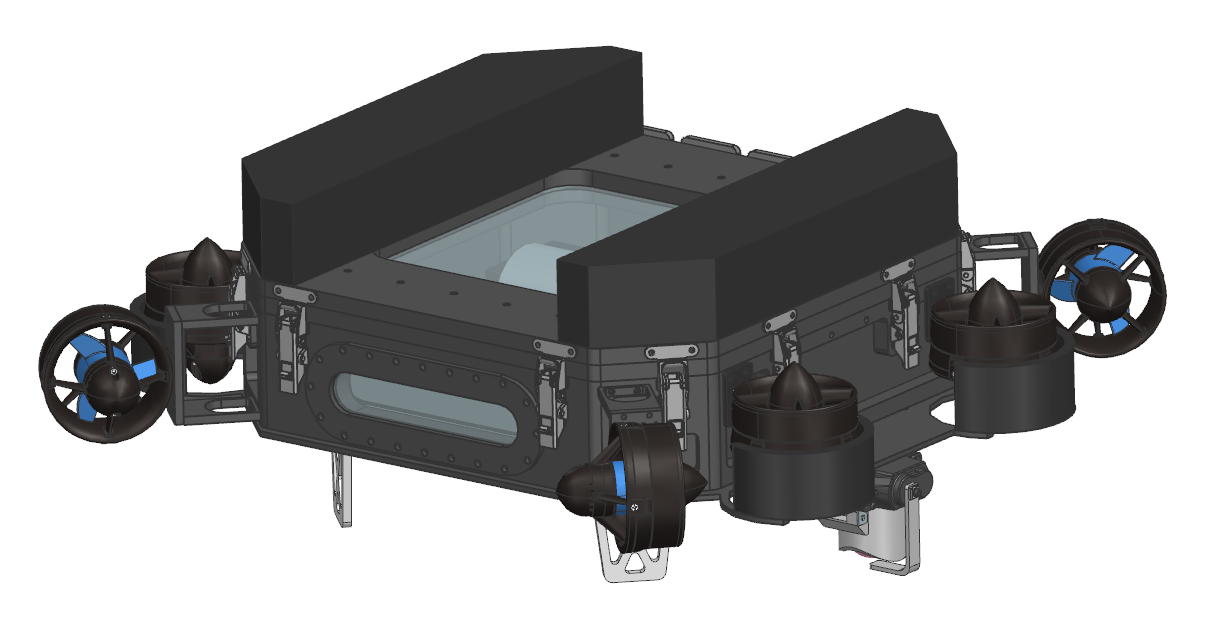
\includegraphics[scale=0.35]{images/Isometric_foam.PNG}}
    \caption{CAD of our 2022-2023 AUV, Argo.}
    \label{fig:sub4}
\end{figure}


\subsection{Other Tasks}
\label{ssec:remaining_tasks}
We plan to attempt one additional task: the bins task. The simplicity of our dropper mechanism makes it quite reliable from a mechanical perspective. However, recognizing the location of the bins requires training another machine learning model, which would be quite difficult. Additionally, due to the need to prioritize higher yield tasks, we were unable to test the dropper, and therefore are unsure of its reliability.  However, our flexibility in tuning movement constants (see \ref{ssec:teleop}), allows us to easily account for changes to Argo’s maneuverability as a result of adding the dropper. Thus, if we are unable to complete this task, we believe it will not affect our ability to complete other tasks.

We do not intend to complete the torpedoes task or any task requiring a grabber. Although we spent some time developing torpedo and grabber mechanical systems, we ultimately decided not to include them in the final iteration of the vehicle. Incorporating either into the vehicle would have taken a significant amount of time away from work on the rest of Argo. Additionally, our hydrophone system is still in development so we would be unable to locate the pinger-based tasks which utilize the torpedo system and grabber.



\section{Design Creativity}
\label{sec:design}


\subsection{Mechanical}
\label{ssec:mechanical}

\begin{figure}[h]
    \centerline{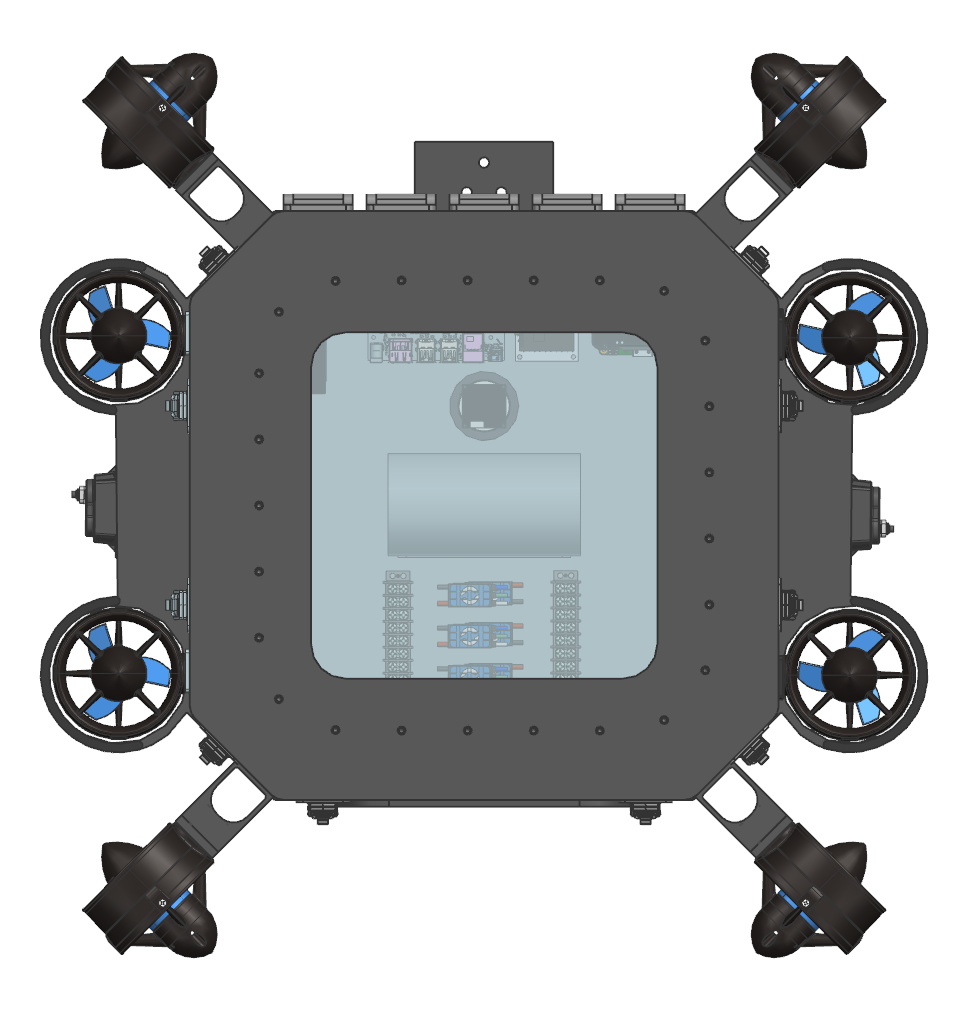
\includegraphics[scale=0.3]{images/Top_no foam.PNG}}
    \caption{CAD of top-view of Argo.}
    \label{fig:sub3}
\end{figure}

\subsubsection{Hull}
\label{sssec:hull}
The hull of Argo was reused from our previous AUV. This hull, which was machined from 6061 aluminum, had provided adequate leak protection for its three ports: a front window for the ZED stereo camera, a window for the bottom camera, and a larger window on the top to make the electrical system visible. A double o-ring face seal was employed at each port to prevent water from being able to enter the interior of Argo. Its eight-thruster configuration had also given it good maneuverability, as it was able to move in all six degrees of freedom. 


In addition to reusing the primary hull component, we incorporated handles to its sides to aid with transport and machined longer legs to make room for the dropper system, which will be discussed in the next subsection. Because Argo’s hull had been designed to allow for modularity, mounting these new components was straightforward. Adding these components increased Argo’s weight, which we dealt with by mounting additional buoyancy foam to the top of the vehicle. To compensate for shifts in Argo’s center of buoyancy, we used the sliding mounts to reposition our four corner-angled thrusters to positions that lent themselves to stable motion. 



\subsubsection{Dropper}
\label{sssec:dropper}

This year, we implemented a marker dropper subsystem. Rather than employing one dropper containing two markers, we incorporated two identical droppers, with one marker in each. This configuration was employed to improve the reliability of the dropper system by eliminating the possibility that two markers would unintentionally be dropped at the same time.
Each dropper consists of a 3D-printed tubular component in which the marker is stored. To hold the marker in place before an intended drop, a sheet metal arm partially blocks the bottom opening of the tube. To release the marker, a servo connected to this arm is actuated, uncovering the bottom opening of the tube and allowing the marker to fall. A sheet metal bracket is used to mount each marker dropper to the sub. 3D-printing large components of the marker droppers was a quick and easy way to produce the complex shapes incorporated into their design. Figure 3 shows a CAD screenshot of a marker dropper assembly while Figure 4 illustrates how each marker dropper was incorporated into the sub.

\begin{figure}[h]
    \centerline{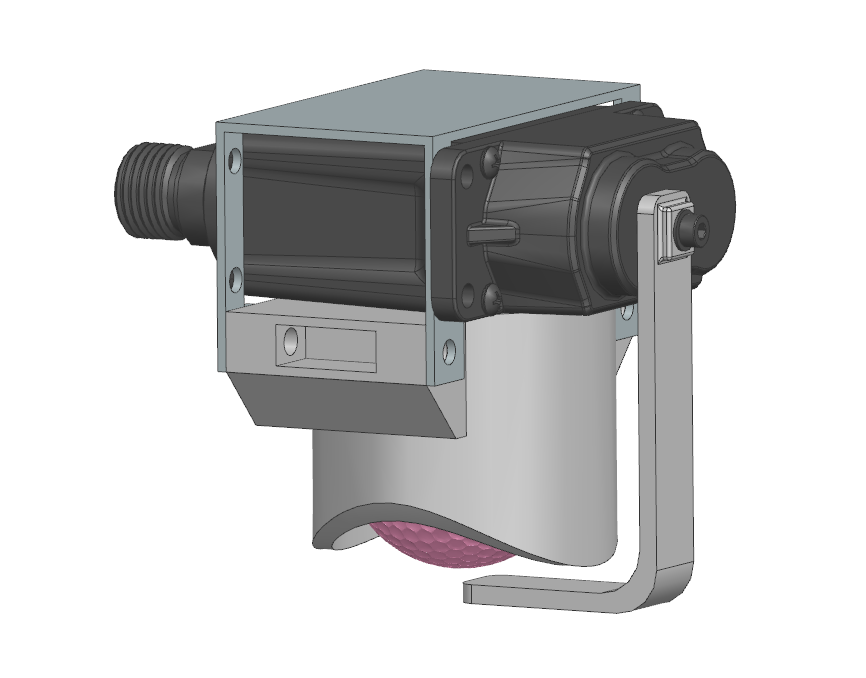
\includegraphics[scale=0.5]{images/Dropper.PNG}}
    \caption{CAD of the dropper mechanism which mounts to the bottom plate of the hull.}
    \label{fig:sub3}
\end{figure}

\begin{figure}[h]
    \centerline{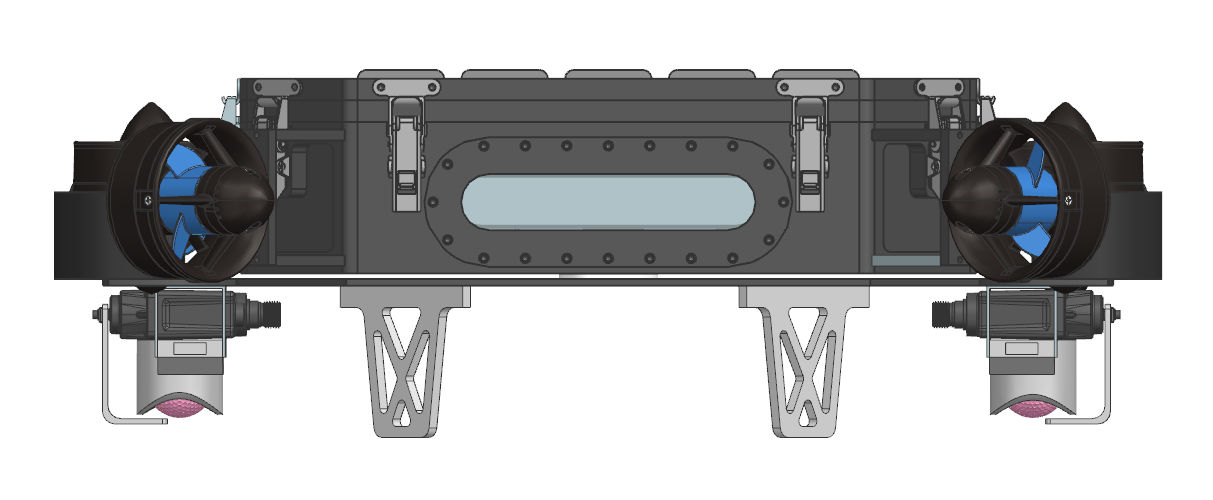
\includegraphics[scale=0.35]{images/Front_no foam.PNG}}
    \caption{CAD of front-view of Argo.}
    \label{fig:sub6}
\end{figure}

\subsection{Electrical}
\label{ssec:electrical}
We continued to iterate on various parts of our electrical system to help meet our goals of flexibility and reliability. Our current power architecture is shown in Appendix B.

\break

\subsubsection{Hall Effect Sensors}
\label{sssec:hall_effects}
To control the behavior of Argo while disconnected from its tether, we used two latching hall effect sensors. They allow us to control the starting, stopping, and resetting of our sensors (in particular, the IMU) without needing a connection to a computer. The hall effect sensors did not require any additional holes in the hull, as powerful magnets are used to switch the states. Being able to quickly control the state of our sensors externally improves the efficiency of our testing setup time. We control the hall effects by wiring them to the main computer and listening for their changes in a control script. Once one of the values changes, an indicator LED is lit so we can see that the state has been activated.

\subsubsection{Motor Control Board}
\label{sssec:motor_board}
Last year, each of our eight thrusters had 3 long wiresr outing across the bottom of the AUV's hull. These 24 wires would connect to eight electronic speed controllers (ESCs) and then output to eight PWM signals. This made the electronics difficult to manage and organize, which is both inconvenient and potentially dangerous. The process to change an ESC was lengthy and prone to breaking other components. As a result, we chose to encapsulate all of these wires and components into a simple printed circuit board. We now have two Motor-ESC boards which each take input from 4 thrusters and output 4 PWM signals. The ESCs connect directly to the PCB with screw-block terminals, so we can easily unscrew and swap them out. The thruster motors and PWM output connect to the PCB using Molex connectors which provide strong connections and can be disconnected easily if needed. This frees space inside Argo for other components and makes swapping easier when necessary.

\subsubsection{Voltage Regulation}
\label{sssec:voltage_regulation}
We continue to use our custom power distribution PCB, which utilizes an off-the-shelf Pololu 5V 15A Step Down Regulator as our DC-DC converter to supply up to 75 W to our system. To upgrade to the Jetson Xavier this year (see \ref{sssec:comp_arch}), we designed a new power regulator to provide the ideal voltage for peak performance on the Jetson Xavier (14V). This mitigates the risk of overvolting the Xavier or having its power input fluctuate over time compared to directly connecting the Xavier to the battery.

    %\paragraph{Power Distribution}
%We continue to use our custom power distribution PCB which steps down the voltage from the battery (16 V)  to our sensors and computational components (5 V). To upgrade to the Jetson Xavier this year, we designed a new power regulator to provide the ideal voltage for peak performance on the Jetson Xavier (14V). This mitigates the risk of overvolting the Xavier or having its power input fluctuate over time compared to directly connecting the Xavier to the battery.


\begin{figure}[htbp]
    \centerline{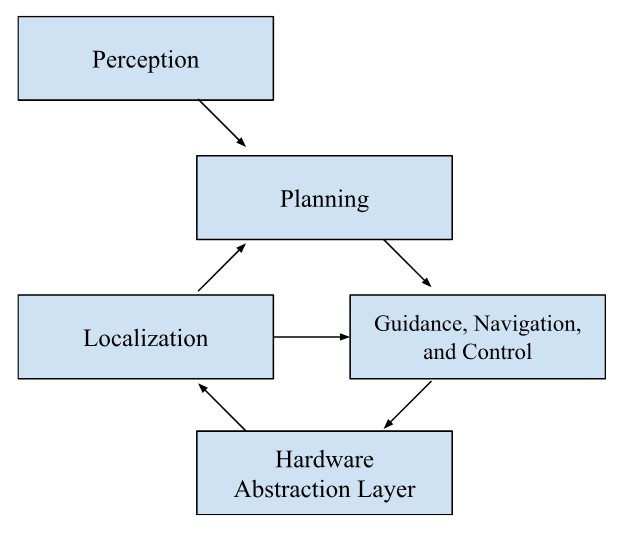
\includegraphics[scale=0.5]{images/ros_diagram.jpg}}
    \caption{High-level Software Architecture}
    \label{fig:ros}
\end{figure}
\subsection{Software}
\label{ssec:software}
Our software stack utilizes the Robot Operating System (ROS) to distribute our logic into distinct modules called nodes. These nodes are organized into packages based on their role in Argo's operation. Fig. \ref{fig:ros} shows these packages, with arrows representing flow of information between packages. The majority of our code is written in Python, with the exception of the hardware abstraction layer, which is written in C. 

\subsubsection{Custom Flight Controller}
\label{sssec:custom_flight_controller}
One of our key priorities this year was the development of a custom flight controller for Argo. While using a PixHawk 4 (PX4) flight controller (see \ref{sssec:comp_arch}) provides some ease of use, it reduces the flexibility of our software system and limits the motion and sensor quality. Therefore, we began developing our own platform with a focus on modularity, customizability, and robustness to address these concerns. For this competition, we are in a transitional phase where most actions are controlled by the PX4 through the MAVROS framework and some are controlled by custom software. This is because we wanted to ensure the flight controller was functional and reliable before use, as it is fundamental to Argo's operation.

\subsubsection{Computing Architecture}
\label{sssec:comp_arch}
We first sought to address the lack of flexibility of the PX4 flight controller. Integrating it into the system required connecting a microprocessor running an operating system (OS) specified by the supplier. While this is a common practice in industry, the issue was that the mandated OS contained many outdated software dependencies. In previous years, we used the same microprocessor to run both our autonomy software and the PX4. However, this became an issue as we were unable to update software dependencies as we developed new software. In response, we designated the PX4 its own microprocessor, allowing us to use any microprocessor, OS, and software for our autonomy stack. This proved invaluable, as we are now able to use a Jetson Xavier NX with the Ubuntu 20.04 operating system without affecting the PX4. This decoupling also will allow us to remove the PX4 from our system in the future without significantly changing the overall architecture or controls software.

\begin{figure}[htbp]
    \centerline{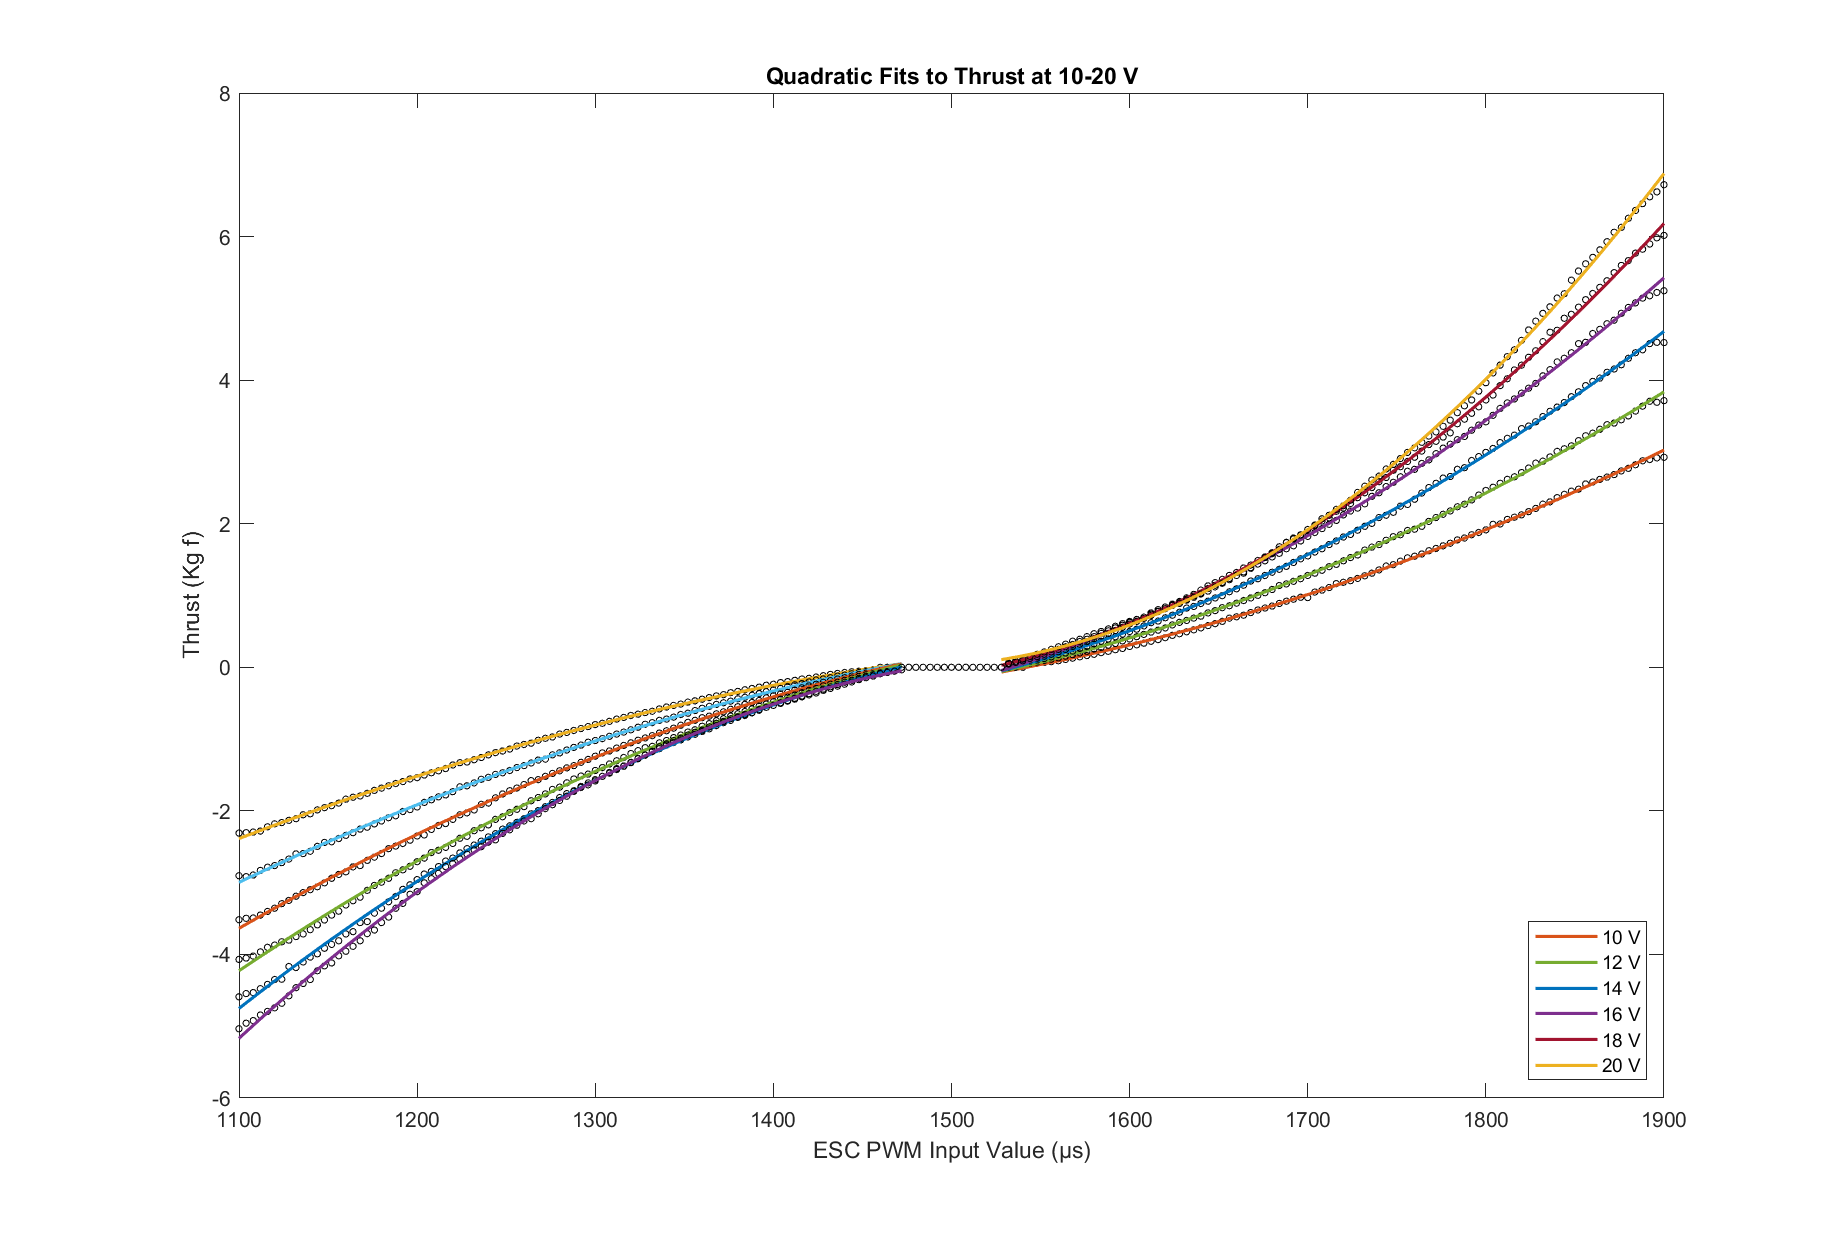
\includegraphics[scale=0.30]{images/motor_profile.png}}
    \caption{Quadratic Fits to Thrust at 10-20 V}
    \label{fig:motor_profile}
\end{figure}

\subsubsection{Motion Control}
\label{sssec:motion_control}
Another issue we wanted to address was the PX4’s limited motion control, given it directly maps motion commands to electrical signals on the motors. This fails to address the physical properties of the motors. These include a nonlinear relationship between the motor’s input signal and output thrust, a difference in maximum thrust when rotating the thruster forwards opposed to backwards, and a deadband in which small signals do not cause the motor to move.
To gain more accurate control of the motion of Argo, we developed a control system that accepts desired thrust as its input. By fitting a quadratic regression model to data provided by the motor specifications, as shown in Figure \ref{fig:motor_profile}, we could accurately map a desired thrust to the corresponding signal to send to the motor. Commanding thrust rather than raw signal allows us to account for the physical properties of the motor that the PX4 alone could not. Because the PX4 does not allow overriding the signal sent to the motor, this system is not currently in use. It is ready for use once the custom flight controller is integrated.

\subsubsection{Depth Sensor Integration}
\label{sssec:depth_sensor}
Last year, data from our depth sensor was read using the PX4. As we aim to remove the PX4 from our system, transitioning to our own custom flight controller requires a different method of processing depth data. This year, we decided to interface with the sensor directly with an Arduino microcontroller via a logic level converter. The microcontroller serializes the data and continuously publishes it to the brain for use within our autonomous routines. This allows us to obtain critical data while keeping our system as modularized as possible and providing the performance and functionality we needed. Benchmarks demonstrated that this method would suffice given our latency requirements. Further testing showed we could have one Arduino microcontroller controlling multiple components, such as our depth sensor and a servo, without significant performance impact.

\subsubsection{Task Planner}
\label{sssec:task_planner}
The task planner is code for coordinating system components to complete tasks during a run. At the previous competition, we used a state machine framework to control our high-level task planner. This framework was useful in the way that it allowed us to reason about our code, but was quite inflexible. This year, we rewrote the framework to allow rapid changes to the task planning logic while at competition.

The goal of the new system was to decouple transitions between states from the state itself. As an example, suppose we decide that attempting to choose a side on the gate is unreliable. In the original logic, the “move towards gate” state would send a “seen glyph” outcome, which would then transition to the “move towards side” state. To make the change, we simply switch the transition to stay in “move towards gate.” This changes the behavior of the task without having to modify any of the business logic of the states.

\subsubsection{Collision Detection}
\label{sssec:collision_detection}
We use PX4 Inertial Measurement Unit (IMU) to detect collisions with the buoy. We only perform collision detection while moving forwards; in order to perform collision detection, we take acceleration measurements along the surge (forwards/backwards) axis of our craft from the IMU, filter out noise, and determine if the negative acceleration exceeds a certain pre-tuned, fixed threshold. Being aware of when the vehicle collides with the buoy is key for being able to hit it twice, as required for maximum points.

\subsubsection{Path Marker Detection}
\label{sssec:path_marker}
In order to detect the pathmarkers located on the bottom of the pool, we use classical computer vision. Our implementation uses the library OpenCV to apply an HSV mask tuned to the color of the marker in the pool, and then runs line detection on the masked output. We then merge similar lines to identify the long edges on opposite sides of the marker, and average their relative angles to find the true heading of the marker relative to the current heading of Argo. 

\subsubsection{Glyph and Object Detection}
\label{sssec:glyph_object_detection}
One advantage of switching our onboard computer is the increased computing power provided by the NX. We now achieve 6 TFLOPS, while last year's system achieved 0.5. We continue to use the ZED 2 Stereo Camera for forward vision and a bottom facing camera for pathmarker detection. 

Having had good results using the YOLOv5 neural network \cite{b3} for object detection last year, we decided to continue to use this model with some modifications to our implementation. Due to our hardware and software upgrades, we were able to fully abandon the deprecated inference network called Darknet. This year we are utilizing the native PyTorch framework which is an open source machine learning framework that is an industry standard for this type of work \cite{b4}. Its ease of use, extensive documentation, and greater usability are much improved compared to our prior framework. With this change, we were able to train our models in a different way as well. We now utilize a service called the Great Lakes Computing Cluster for all of the computational power for generating the model, and it allows us to train our models in a fraction of the time.

\subsubsection{Machine Learning Process}
\label{sssec:ml_flow}
In line with our goal to increase our system’s ability to rapidly iterate designs, we focused on overhauling and documenting the workflows we use to train deep learning models and collect data. 

Previously, our training process consisted of a complicated series of manual steps that required extensive time and knowledge of the system. In response, we developed a series of scripts to automate the setup of training on the Great Lakes Computing Cluster and removed the need to generate the image labels for each training run. Since the contents of a label file are static after bounding boxes are drawn on each image, we simplified the process by caching them instead of re-generating them every time. To understand how well newly trained models perform on a test set, we utilized a model evaluation script, provided by the Ultralytics YOLO package. These evaluation metrics allow us to easily compare the performance of two models.

The data collection process was similarly suboptimal. We created a data pre-processing script that ensures all of the images were of the correct resolution, file type, and naming convention. We would then import the images to LabelBox and draw bounding boxes. A second script then generates the label files and splits them into the required train and test designations. Finally, we are left with two separate folders for training and testing, each containing unique images and labels. This system automates the process for transforming raw data into labeled training data which saves time and improves effectiveness.

\section{Testing and Experimental Results}
\label{sec:testing}

\subsection{Teleoperation Framework}
\label{ssec:teleop}
A key takeaway from competing in-person last year was the need for an efficient water testing infrastructure. Due to the interdependence of our subsystems, it is challenging to test individual components of our system while Argo is operating autonomously; it is often difficult to diagnose the source of errors when the entire system is running. This past year, we developed a robust teleoperation (teleop) framework that allows a human driver to manually control various aspects of Argo while other subsystems run autonomously, enabling us to quickly and efficiently execute unit tests and debug components in isolation.

Our teleop framework makes significant improvements to the default manual control system provided by ArduSub on our Pixhawk flight controller. The ArduSub manual control system required all components to be driver-controlled or autonomous at once, which limited our testing capabilities. With our new teleop framework, we are able to dynamically toggle the control mode of individual components, making our testing process much more fluid. With our new system, we were able to reduce the time required to switch between control modes from thirty seconds to nearly instantaneous. In order to halt Argo in an emergency situation, the ArduSub manual control system required many human inputs to our base-station. Our system has a straightforward emergency stop button, allowing us to quickly stop all processes and minimize potential damage to Argo or the environment.

A significant benefit of our new teleop framework is the ability to efficiently tune Argo’s control parameters and to observe the Argo’s movement capabilities in a controlled environment. At last year’s RoboSub competition, we tuned the control parameters of each degree of freedom separately. While this made the process more efficient, we found that the accuracy of Argo’s movements would decline significantly when performing compound motions autonomously (i.e. moving forward and turning at the same time). With our new teleop framework, we can tune, for example, our depth controller while manually maneuvering Argo. This provides a much more precise sense of how Argo will move while performing tasks autonomously.


\subsection{In-Water Testing}
\label{ssec:in_water_testing}

At the 2023 RoboSub competition, we encountered numerous problems while the AUV was running in-water that we feel we could have resolved with more water testing throughout the year. This past year, our team has made a concerted effort to utilize the resources available through our university to perform as much in-water testing as possible. We used a water tank in the Ford Motor Company Robotics Building (FMCRB) at the University of Michigan to perform unit tests and sensor, motor, and camera calibrations. We performed control parameter tuning and movement testing at the U-M Marine Hydrodynamics Laboratory (MHL). We performed larger-scale tests that involved competition elements such as the gate at the Dexter Community Pool in Dexter, MI.

Before each in-water testing session, we wrote a test plan which describes what specific tests are to be carried out and explains the high-level purpose of each test. We recorded the procedure for each task and the expected results, along with some notes on potential problems or bugs. This simple addition to our testing workflow allowed us to streamline testing once we arrived on-site and allowed us to create a log of tests we’ve previously performed and issues we’ve previously encountered. See Appendix C for a sample test plan. 

Throughout the Fall semester this past year, we significantly overhauled our software architecture and performed some mechanical changes to Argo. During this time, we primarily performed smaller unit-tests using the water tank at the FMCRB. Once our software system was stable during the Spring semester, we were able to perform many more in-water tests at the MHL and the Dexter Community Pool. Over the course of the Spring semester, we typically performed between two and four water tests per month. Once classes ended in May, we were able to increase the frequency of water testing to roughly twice a week.

As we incrementally added new components to the hull of Argo, such as the redesigned legs and dropper mechanisms, we assessed how they affected the modified weight distribution, movement, and PID tuning of Argo using several in-water unit tests. These included driving in a square and driving forward, both at a set depth. With our new teleop framework, this sort of movement testing was made more efficient.

While in-water testing sessions were primarily used to test software changes and the efficacy of Argo to perform competition tasks, we also used these tests to gain feedback about Argo's mechanical design. One key takeaway from our various tests earlier in the year was the need to properly reinforce our mechanical components to protect them from collisions. For example, as we iterated on the design of our dropper mechanism, we realized that it was easy for the mechanism to unintentionally collide with the floor of the pool. Once we understood this problem, we were able to reposition the dropper mechanism and add metal guards to protect it from damage.

We performed testing with competition elements and filmed the pre-qualification video at the Dexter Community Pool. An indoor pool environment made it much easier to manipulate competition elements to simulate a competition environment. In particular, we performed testing of the gate and buoy tasks by securing the elements to the bottom of the pool with weights.


\subsection{Off-Board Testing}
\label{ssec:off_board_testing}
In order to write, execute, and test our software off of Argo, we developed Docker images that emulate our companion computer, the PX4, and the MAVROS environment. This workflow allows anyone on our team to set up our development environment on their computer in just a few steps. In general, we tested the logic of our software off-board of Argo and reserved in-water testing for collecting data to improve our vision system or test the physical results of the algorithms once they had been tested in simulation. This prevented valuable in-water testing time from being consumed with simple software errors.

We also developed a Unity simulation that communicates with our software emulation in Docker, We wrote Unity C\# software to simulate the movement, sensor data, and vision data of Argo with random statistical noise. The simulation also enables us to evaluate our software's behavioral logic within a to-scale Transdec scene created by Team Inspiration (see Fig. \ref{fig:unity}).

To visualize the output of our software both in Docker and on the real AUV, we created visualizations using RQt, a ROS dashboard library. We leveraged RQt to graph data and dynamically tune control parameters, allowing for easy incremental testing.

    \begin{figure}[htbp]
    \centerline{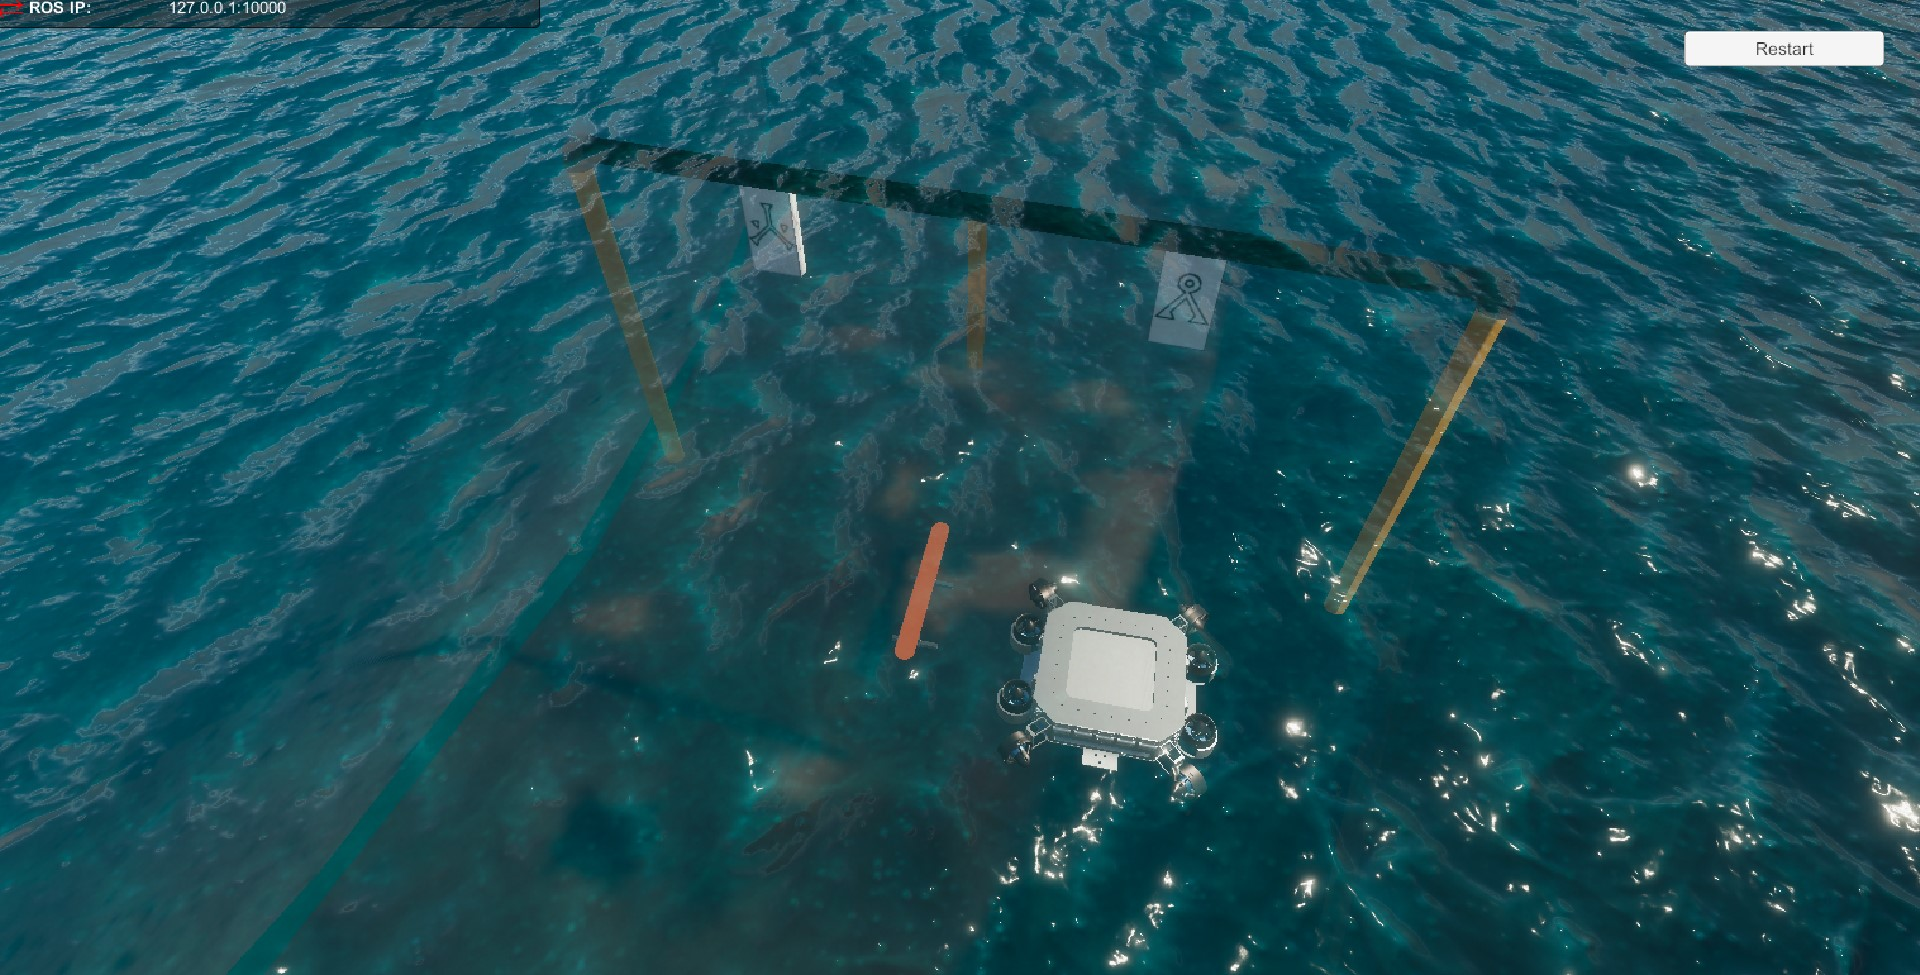
\includegraphics[scale=0.2]{images/unity_new.jpg}}
    \caption{Testing the gate task logic using Docker and Unity.}
    \label{fig:unity}
    \end{figure}

\section*{Acknowledgements}

The Michigan Robotic Submarine team would like to thank our 2023 sponsors for their monetary support: Ford Motor Company, Aptiv, Siemens, along with the University of Michigan College of Engineering and Central Student Government. In addition, we would like to thank our advisor Dr. Katie Skinner for continuously supporting our team by advising us and overseeing the Multidisciplinary Design Program which allows members to earn class credit for their contributions to our team.

We are greatly appreciative of the Marine Hydrodynamics Lab staff, especially Jim Smith and Jason Bundoff, for graciously providing the team with an in-water testing location. 

We also would like to thank the Wilson Student Team Project Center facilities and Ford Motor Company Robotics Building staff, especially Alyssa Emigh and Chris Gordan, for hosting our team workspace, providing tools and resources, and overall supporting our endeavors. 

We are also thankful of Mariah Moss and Katelyn Killewald from the Office of Student Affairs at the University of Michigan College of Engineering for their guidance in developing our team and assistance purchasing the materials that make our work possible. 

Lastly, we would like to thank the RoboNation team for organizing the RoboSub competition. We are also thankful for the hydrophone and image data provided through the RoboNation data sharing program.

\begin{thebibliography}{00}
\bibitem{b1} Inspiration Robotics, ``RoboSub-Simulation". Github.com. https://github.com/InspirationRobotics/RoboSub-Simulation (accessed June 11, 2022)
\bibitem{b2} A. Zelenak, ``A PID controller for ROS". bitbucket.org. https://bitbucket.org/AndyZe/pid/src/master/ (accessed June 11, 2022)
\bibitem{b3} G. Jocher, ``ultralytics/yolov5: v6.1 - TensorRT, TensorFlow Edge TPU and OpenVINO Export and Inference”. Zenodo, Feb. 22, 2022. doi: 10.5281/zenodo.6222936.
\bibitem{b4}{P. Adam et al., ``PyTorch: An Imperative Style, High-Performance Deep Learning Library", in Advances in Neural Information Processing Systems 32, Curran Associates, Inc., 2019, pp. 8024–8035.}

\end{thebibliography}

\clearpage
\appendices
\section{Sample Test Plan}
The following is a test plan from a testing session at the MHL on February 3rd, 2023. It has been adapted for formatting and clarifying comments have been placed in brackets. \\

\subsection{Primary Tasks}
\begin{itemize}
    \item Drive around
    \item Tune heave PID [heave is the up/down axis]
    \item Tune yaw PID [yaw is the heading axis]
\end{itemize}

\subsection{Drive around}
\subsubsection{Procedure}
\begin{itemize}
    \item Boot up sub
    \item SSH into pi’s and start up services
    \item Connect to QGroundControl
    \item Set SYS ID = 1 and drive around sub
\end{itemize}
\subsubsection{Expectation}
\begin{itemize}
    \item Sub should be able to be driven around the MHL normally
\end{itemize}
\subsubsection{Results}
\begin{itemize}
    \item Expectation met
\end{itemize}

\subsection{Test heave}
\subsubsection{Procedure}
\begin{itemize}
    \item Start depth launch file [a launch file is a utility provided by ROS to start related systems simultaneously]
    \item Start teleop launch file
\end{itemize}
\subsubsection{Expectation}
\begin{itemize}
    \item Sub should approach and remain at depth
\end{itemize}
\subsubsection{Results}
\begin{itemize}
    \item Some overshoot but stabilizes pretty well (see recorded data) [data was collected using rosbag, a utility which records published messages. Unfortunately, this data is stored in a binary format not amenable to sharing]
\end{itemize}

\subsection{Test yaw}
\subsubsection{Procedure}
\begin{itemize}
    \item Start depth launch file
    \item Start yaw launch file
    \item Start teleop launch file
\end{itemize}
\subsubsection{Expectation}
\begin{itemize}
    \item Sub should approach and remain at yaw
\end{itemize}
\subsubsection{Results}
\begin{itemize}
    \item Stabilizes pretty well (see recorded data)
    \item Noticeable drift on IMU (see action items)
\end{itemize}

\subsection{Overall notes}
\begin{itemize}
    \item PID tuning with dashboard works very well on one base station
    \item Dependency issues on the other
    \item Switch power cable is delicate, needs to be positioned certain way to work well
    \item Teleop launch files may have some minor bugs
    \item PixHawk IMU drifts significantly
    \item Need solution to better EStop the sub
    \item Collected rosbags of MAVROS topics
\end{itemize}

\subsection{Action items}
\begin{itemize}
    \item Thruster came off – needs to be fixed (urgent)
    \item Fix package issues on other base station [the team has two base stations we use for testing]
    \item Fix network switch
    \item Re-mount AHRS
    \item Check drift on PixHawk
    \item Purchase software EStop button, look into necessary code
\end{itemize}
\raggedbottom

\pagebreak
\section{Power Architecture}

% \vspace{0.5cm}
% 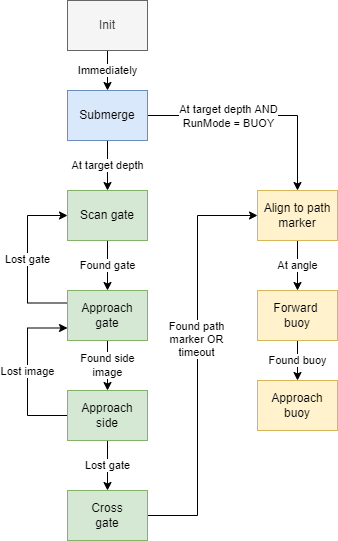
\includegraphics[scale=0.6]{images/task_state_machine.png}

\vspace{0.5cm}
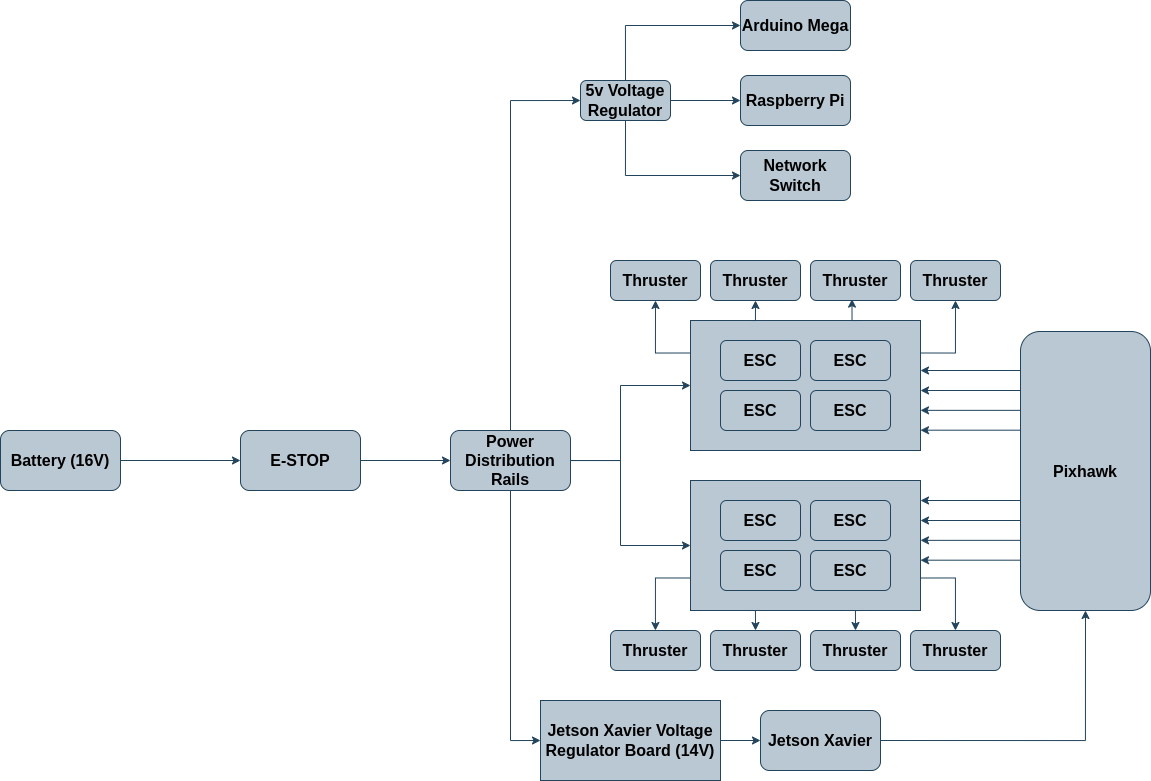
\includegraphics[scale=0.45]{images/power.png}
\newpage

\clearpage
\section{Component Specifications}

\begin{center}
\begin{table}[htbp]
\begin{tabularx}{\textwidth}{|X|X|X|X|X|X|}
    \hline
        Component & Vendor & Model/Type & Specs & Cost (if new) & Year of Purchase \\ \hline
        ASV Hull Form/Platform  & American Tooling \& Prototype & Custom & 6061 Aluminum & \$3250.00 & 2022 \\ \hline
        Waterproof Connectors & Blue Robotics & Potted cable penetrators & 25mm long M10x1.5 for 6mm cable & \$120.00 & 2020 \\ \hline
        Propulsion  & Blue Robotics & T200 w/ Propellor & 7-20V & \$1,074.00  & 2020\\ \hline
        Power System & N/A & Custom & N/A & N/A & N/A \\ \hline
        Motor Controls  & Blue Robotics & Basic ESC & 7-26V & \$172.00  & 2023 \\ \hline
        CPU & Nvidia & Jetson Nano & Quad-core ARM A57 @ 1.43 GHz, 4 Gb RAM & \$110.00  & 2021 \\ \hline
        Compass  & PixHawk & PX4 & Accel/Gyro: ICM-20689 with Magnetometer & \$189.99  & 2022 \\ \hline
        Inertial Measurement Unit (IMU)  & PixHawk & PX4 & MPU6000 9-axis & 189.99 & 2022 \\ \hline
        Doppler Velocity Log (DVL) & N/A & N/A & N/A & N/A & N/A \\ \hline
        Camera(s) & Stereolabs, Blue Robotics & ZED2, Low-light HD USB Camera & stereo vision, pathmarker detection & \$449.00, \$99.00  & 2020, 2021 \\ \hline
        Hydrophones & N/A & N/A & N/A & N/A & N/A \\ \hline
        Localization and Mapping  & N/A & Custom & N/A & N/A & N/A \\ \hline
        Vision  & N/A & YOLOv5, PyTorch, OpenCV & train convolutional neural network and perform classical computer vision & N/A & 2023 \\ \hline
        Localization and Mapping  & N/A & Custom & N/A & N/A & N/A \\ \hline
        Autonomy  & N/A & Custom & N/A & N/A & N/A \\ \hline
        Open source software & N/A & Andy Ze ROS PID & PID Control & N/A & N/A \\ \hline
    \end{tabularx}
\label{tab1e}
\end{table}
\end{center}


\end{document}
